\chapter{Introduction}
\begin{figure}
\centering
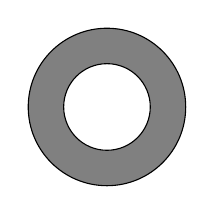
\begin{tikzpicture}[scale=.25]
  \filldraw[draw=black,fill=gray] (0,0) circle [radius=4];
      \filldraw[draw=black,fill=white] (0,0) circle [radius=2.2];
 \end{tikzpicture}      
 \hspace{.5cm}
\begin{tikzpicture}[scale=.25]
    \foreach[count=\p] \x / \y in \data { 
	\node[draw, circle, scale=.25, fill=white](\p) at (\x, \y) {};
    } 
 \end{tikzpicture}
 \caption{Point Cloud sampled from annulus}
 \end{figure}
Over the past twenty years \emph{topological data analysis} has been found to be very useful in understanding scientific data. The primary tools of the field: persistent homology and mapper have been used in image processing, chemistry, astronomy, business, and medicine. The dichotomy with traditional data analysis, in which one concerns itself with modeling physical phenomena from measurements on finite sets of samples, is that in topological data analysis, one assumes that the input point cloud comes from an unknown underlying geometric space. Topological data analysis then focuses on the recovery of the lost topology of this underlying space \cite{c-tnd-09}. In this thesis we aim to make the primary tool for topological data analysis, persistent homology, computable for practitioners. To this end we investigate parallel algorithms for the computation of persistent homology. We present two new parallel algorithms for persistence, the first for computing homology, and the second which extends it to the persistent setting. We connect these procedures to \emph{spectral sequences} a manual calculation tool used by mathematicians for computing algebraic structures by hand.
\section{Background}
Suppose someone asked you describe the shape of this point cloud. One might be inclined to propose that the point cloud looks quite disconnected. Indeed, the topology of a set of points in $\R^n$ is not all that interesting. Perhaps, however, if you were to squint your eyes, you might be inclined to describe the shape as something like an annulus. Persistence is a tool for modeling this phenomenon. As an example, for any \emph{metric space} $(X,d)$ and  $\epsilon > 0$ we can define a space: \[ M_\epsilon = \bigcup_{x \in X} B_{\epsilon}(x) \] where $B_{\epsilon}(x) = \{ y \mid d(x,y) < \epsilon\} $ is the \emph{ball of radius $\epsilon$ around x}. Notice that by varying the scale parameter $M_\epsilon$ has different topologies. The collection $\{M_\epsilon\}_\epsilon$ of spaces together with the inclusion maps between $M_\epsilon$ and $M_{\epsilon'}$ for any $\epsilon < \epsilon'$ is called a \emph{one parameter family} of spaces.   
 
 \begin{figure}
\centering
 \hspace{.5cm}
 \begin{tikzpicture}[scale=.25]
\begin{pgfonlayer}{ball}
      \foreach[count=\p] \x / \y in \data {
         \fill[gray!50,radius= .3 cm] (\x,\y) circle{};
	}
 \end{pgfonlayer}{ball}
	\foreach[count=\p] \x / \y in \data {
	 \node[draw, circle, scale=.25, fill=white](\p) at (\x, \y) {};
	 }
\end{tikzpicture}
 \hspace{.25cm}
\begin{tikzpicture}[scale=.25]
\begin{pgfonlayer}{ball}
      \foreach[count=\p] \x / \y in \data {
         \fill[gray!50,radius= .6 cm] (\x,\y) circle{};
	}
 \end{pgfonlayer}{ball}
	\foreach[count=\p] \x / \y in \data {
	 \node[draw, circle, scale=.25, fill=white](\p) at (\x, \y) {};
	 }
\end{tikzpicture}
 \hspace{.25cm}
\begin{tikzpicture}[scale=.25]
\begin{pgfonlayer}{ball}
      \foreach[count=\p] \x / \y in \data {
         \fill[gray!50,radius= 1 cm] (\x,\y) circle{};
	}
	\fill[gray!50,radius= 2.4 cm] (0,0) circle{};
 \end{pgfonlayer}{ball}
	\foreach[count=\p] \x / \y in \data {
	 \node[draw, circle, scale=.25, fill=white](\p) at (\x, \y) {};
	 }
\end{tikzpicture}
\caption{Model spaces at various scales}
\end{figure}

 Persistent topology concerns itself with topological features which can be found at multiple scales.

\section{Preliminaries}
We begin with a review of algebraic topology. 
We refer the reader to Hatcher for background material in algebraic topology~\cite{hatcher}.

A \emph{simplicial complex} is a collection $\K$ of finite sets called
\emph{simplices} such that if $\sigma \in \K$ and $\tau \subseteq \sigma$ then 
$\sigma \in \K$. We say that $\tau$ is a \emph{face} of $\sigma$, its \emph{coface}. A simplex
is \emph{maximal} if it has no proper coface in $\K$. The set of maximal cells of a 
simplicial complex $\K$ is $\M(\K)$. If $\card{\sigma} = k+1$
then $\sigma$ is a $k$-simplex, it has \emph{dimension} $k$, denoted 
$\dim{\sigma} = k$. We say that $\K$ is \emph{$d$-dimensional} if 
$d = \max_{\sigma \in \K} \dim{\sigma}$. 

Suppose we have a subset $L \subseteq K$.  $L$ is a \emph{subcomplex}
if it is a simplicial complex. The \emph{closure} of $L$ is 1
$\Cl(L) = \{ \tau \mid \tau \subseteq \sigma \in L\}$ and it is a simplicial complex. The 
\emph{$k$-skeleton} of a complex $\K$ is the set of all simplices
of dimension less than or equal to $k$. Note that the 1-skeleton of
any complex is as a graph.

Let $\Delta^n$ be the $n$-simplex defined on $[n+1]$.  We note that 
$\Delta^n$ is traditionally defined in a geometric setting and is
called the \emph{standard $n$-simplex}~\cite{hatcher}, although we 
are using an abstract version here for our purposes. For any
\emph{indexing set} $J \subseteq [n]$, $\Delta^J$ is the $(\card{J}-1)$ 
dimensional face of $\Delta^n$  that is defined on $J$.

We define a \emph{filtration} of topological spaces to be a finite sequence of topological spaces connected by
continuous maps. Given a filtration of simplicial complexes, whose final space is $\K$ we can create a  
partial ordering on the simplices of $\K$ such that the $i^{th}$ prefix of the ordering is the image in $\K$ of the $i^{th}$ map. Each prefix is itself a subcomplex of $\K$, so in practice we consider only filtrations of spaces connected by inclusion maps.

Given a simplicial complex $\K$, An \emph{open cover} of $\K$ is a collection of subsets $\{C_i\}_i$ of $\K$ where the union of the $C_i$ is $\K$. Similarly, we call a cover closed if each element of the cover is a subcomplex. 

The \emph{nerve} $\N(\C)$ of a cover $\C$ is the simplicial complex on $[\card{\C}-1]$ whose $k$-simplices 
represent the non-trivial intersections of subsets of $\C$ of size $k+1$. The nerve is a subcomplex of the standard $n$-simplex and so we may denote its simplices by $\Delta^J$ where $J \subseteq [\card{\C}-1]$. 

It is sometimes convenient to encode the cover $\C$ as a map $N: \K \rightarrow \Delta^[\card{\C}]$ where each 
simplex $\sigma \in \K$ is mapped to the list of the cover sets containing $\sigma$.

A simplicial complex may be viewed as the result of gluing simplices of 
different dimensions along common faces. Other types of complexes are defined 
similarly using different types of \emph{cells}. Such \emph{cellular} complexes include \emph{cubical} complexes, \emph{simplicial sets}. $\Delta$-complexes, and \emph{CW-complexes}, 
to name a few~\cite{ez-ssc-50,hatcher,kmm-ch-04,m-soat-68}. 

\section{Homology}
In this section, we describe the homology of cellular spaces over 
field coefficients. Homology, however, is an invariant of arbitrary topological 
spaces and may be computed over arbitrary coefficient rings~\cite{hatcher}.  
Suppose we are given a finite cellular complex $\K$ and a field $k$. 
The \emph{$n$th chain vector space $C_n$} is the $k$-vector space generated by 
the set of $n$-dimensional cells of $K$, its \emph{canonical basis}.  
Suppose we are given a linear \emph{boundary operator} 
$\bd_n\colon C_n \rightarrow C_{n-1}$ such that 
$\bd_n \circ \bd_{n-1} \equiv 0$ for any $n$.  
The boundary operator connects the chain vector space into a 
\emph{chain complex $C_*$}:
\begin{equation*}
  \cdots \rightarrow             C_{n+1}
         \xrightarrow{\bd_{n+1}}  C_n
         \xrightarrow{\bd_n}     C_{n-1}
         \rightarrow \cdots .
\label{eqn:chaincomplex}
\end{equation*}
Given any chain complex, the \emph{$n$th homology vector space $H_n$} is:
\begin{equation}
  \label{eqn:homology}
  H_n = {\ker{\bd_n}}\,/\,{\im{\bd_{n+1}}}, 
\end{equation}
where $\ker(.)$ and $\im(.)$ are the \emph{kernel} and \emph{image} of $\bd$, 
respectively.
Each homology vector space is characterized fully by its \emph{Betti number}, 
$\betti_n = \dim{H_n}$.  
We now only need to define boundary operators to get homology. 
For simplicial homology, we begin by defining the action of the boundary operator on any
$n$-simplex $[v_0,\ldots,v_n] \in \K$:

\begin{equation*}
\bd_n [v_0,\ldots,v_n] = \sum_i (-1)^i [v_0,\ldots,\hat{v_i},\ldots,v_n],
\end{equation*}
where $\hat{v_i}$ indicates that $v_i$ is deleted from the vertex 
sequence. The boundary operator is the linear extension of the above action.

Over field coefficients, homology is a vector space characterized by its dimension, 
so we may compute homology using \emph{Smith Normal Form}~\cite{uhlig}, a matrix reduction technique 
similar to Gaussian Elimination~\cite{uhlig}. However, because we reduce boundary matrices and not general matrices, we may perform specific optimizations to improve the practical running time of these procedures. 
The original modified algorithm is referred to as the persistence algorithm~\cite{elz-tps-02,zc-cph-05}. 
\section{Persistent Homology}
